\documentclass[aspectratio=169]{beamer}
\usepackage{graphicx}

\title{Deep G-Buffers for stable Global Illumination Approximation}
\author{Ferit Tohidi Far}
\usetheme{Frankfurt}

\begin{document}
	\maketitle

	\begin{frame}
		\frametitle{Content}
		\begin{itemize}
			\item Global illumination
				\begin{itemize}
					\item Pathtracing
					\item Visual effects
					\item Radiosity
					\item Inefficiency
				\end{itemize}
			\item Traditional rendering
				\begin{itemize}
					\item Forward rendering
					\item Deferred rendering
				\end{itemize}
			\item Deep G-Buffers)
				\begin{itemize}
					\item Benefits
					\item Generating 2-layer deep g-buffer
					\item Global illumination approximation
				\end{itemize}
		\end{itemize}
	\end{frame}

	\begin{frame}
		\frametitle{Global illumination}
		\begin{itemize}
			\item lighting of a scene
			\item direct \textbf{and indirect} light is considered
			\item causes visual effects that convey realism
			\item most popular method is pathtracing
		\end{itemize}
	\end{frame}

	\begin{frame}
		\frametitle{Pathtracing}
		\begin{itemize}
			\item monte-carlo simulation
			\item send camera ray through each pixel
			\item allow ray to reflect \textbf{diffusely or specularly}
			\item trace it back to a light source
			\item if a light source was hit, the pixel is colored (albedo of hit-object)
			\item else the pixel is black (in shadow)
			\item each pixel is sampled thousands of times, then averaged
		\end{itemize}
	\end{frame}

	\begin{frame}
		\frametitle{Visual effects}
		\begin{center}
			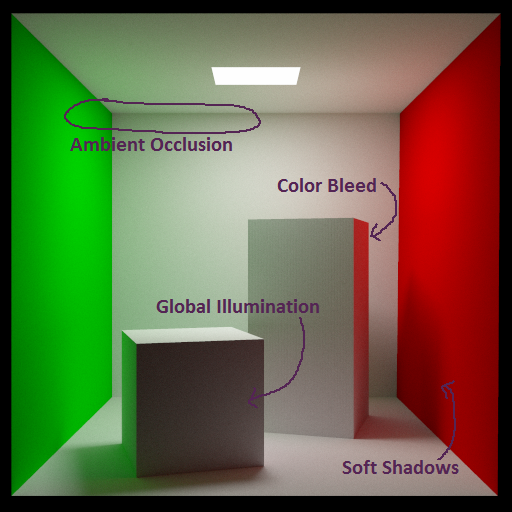
\includegraphics[width=.7\textwidth]{img/visual_effects.png}
		\end{center}
	\end{frame}

	\begin{frame}
		\frametitle{Radiosity}
		\begin{itemize}
			\item scene is divided into patches
			\item each patch is a light receiver and emitter 
			\item initialize scene with at least one patch that emits non-zero amount of light
			\item iteratively update receivance and emitance of each patch
			\item \textbf{purely diffuse global illumination}
		\end{itemize}

		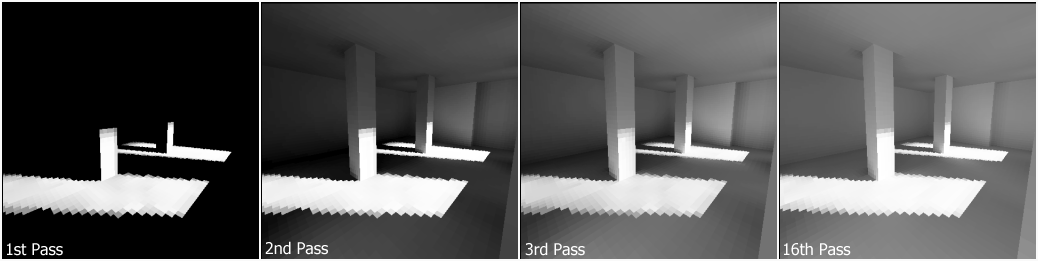
\includegraphics[width=\textwidth]{img/radiosity.png}
	\end{frame}

	\begin{frame}
		\frametitle{Inefficiency}
		\begin{itemize}
			\item pathtracing 
				\begin{itemize}
					\item computes multiple ray bounces
					\item requires thousands of samples (probably more) 
				\end{itemize}
			\item radiosity
				\begin{itemize}
					\item needs large amount of patches for good results
					\item has to be recomputed if an object moves
				\end{itemize}
			\item both cannot be computed in real-time (yet)
		\end{itemize}
	\end{frame}

	\begin{frame}
		\frametitle{Traditional rendering}
		\begin{itemize}
			\item rasterization
			\item way easier to compute than raytracing
			\item interactive framerates
			\item trade-off: not as realistic
			\item requires techniques to simulate visual effects
		\end{itemize}
	\end{frame}

	\begin{frame}
		\frametitle{Forward rendering}
		\begin{itemize}
			\item computes lighting in a single pass:
				\begin{itemize}
					\item for each fragment compute lighting
					\item do z-test
					\item render to frame-buffer or discard accordingly
					\item render frame-buffer to screen
				\end{itemize}
			\item computes lighting for fragment regardless if visible or not
		\end{itemize}
	\end{frame}

	\begin{frame}
		\frametitle{Deferred rendering}
		\begin{itemize}
			\item computes geometry (stored in g-buffer) in first pass:
				\begin{itemize}
					\item albedo-buffer
					\item normal-buffer
					\item z-buffer
				\end{itemize}
			\item render g-buffer to texture-buffer
			\item compute lighting in second pass:
				\begin{itemize}
					\item read frontmost scene geometry from g-buffer
					\item compute lighting
					\item render to screen
				\end{itemize}
			\item only computes lighting for visible fragments
		\end{itemize}
	\end{frame}

	\begin{frame}
		\frametitle{Deep G-Buffers}
		\begin{itemize}
			\item generate 2-layer deep g-buffer with depth-peeling or oracle
			\item enforce minimum depth separation
			\item consider second layer for visual effects
		\end{itemize}
	\end{frame}	

	\begin{frame}
		\frametitle{Generating a 2-layer deep g-buffer (depth-peeling)}
		\begin{itemize}
			\item \textbf{depth-peeling method}
			\item collect first layer g-buffer as usual
			\item compute second layer g-buffer by stripping the first layer
			\item takes two passes over scene geometry\pause
			\item instead use oracle and do it in a single pass!
		\end{itemize}
	\end{frame}	

	\begin{frame}
		\frametitle{Generating a 2-layer deep g-buffer}
		\begin{itemize}
			\item \textbf{use some oracle to predict first layer z-buffer}
			\item remember that we are running some simulation/animation
			\item frames are computed per time-step
			\item after a time-step, the object locations won't change \textbf{that much}
			\item we even have knowledge of position and velocity updates
			\item exploit this by recycling information from the previous frame and adjusting it a little
			\item 4 different variants available
			
		\end{itemize}
	\end{frame}	

	\begin{frame}
		\frametitle{Generating a 2-layer deep g-buffer (previous variant)}
		\begin{itemize}
			\item \textbf{previous variant}
			\item recycle first layer z-buffer of previous frame
			\item the smaller the position updates, the smaller the error
			\item even then, errors would only appear in the second layer (invisible unless transparent)
			\item does not guarantee minimum separation
		\end{itemize}
	\end{frame}	

	\begin{frame}
		\frametitle{Generating a 2-layer deep g-buffer (delay variant)}
		\begin{itemize}
			\item \textbf{delay variant}
			\item introduce a frame of latency
			\item frame and animation/simulation are out of sync by one frame
			\item use first layer z-buffer of precomputed latency frame 
			\item drawback: one frame of latency
		\end{itemize}
	\end{frame}	

	\begin{frame}
		\frametitle{Generating a 2-layer deep g-buffer (predict variant)}
		\begin{itemize}
			\item \textbf{predict variant}
			\item use velocities from animation/simulation
			\item predict position updates of objects
			\item 
		\end{itemize}
	\end{frame}	

	\begin{frame}
		\frametitle{Generating a 2-layer deep g-buffer (reproject variant)}
		\begin{itemize}
			\item \textbf{reproject variant}
			\item performs minimum separation test against previous frame's first layer z-buffer
			\item visibility test done using previous z-buffer ("in the past")
			\item same source of error as predict variant, but not as bad (velocities are perfect)
			\item delivers most stables performance out of the 4 variants
			
		\end{itemize}
	\end{frame}	

	\begin{frame}
		\frametitle{Global illumination approximation using Deep G-Buffers}
		\begin{itemize}
			\item compute ambient occlusion 
			\item compute some radiosity steps
			\item compute screen space reflections
			\item apply direct and ambient light
		\end{itemize}
	\end{frame}	

	\begin{frame}
		\frametitle{Ambient occlusion with Deep G-Buffers}
		\begin{itemize}
			\item 
			
		\end{itemize}
	\end{frame}	

	\begin{frame}
		\frametitle{Reflections with Deep G-Buffers}
		\begin{itemize}
			\item 
			
		\end{itemize}
	\end{frame}	

	\begin{frame}
		\frametitle{Radiosity with Deep G-Buffers}
		\begin{itemize}
			\item temporal filtering for undersampling noise reduction
			
		\end{itemize}
	\end{frame}	

	\begin{frame}
		\frametitle{Results}
		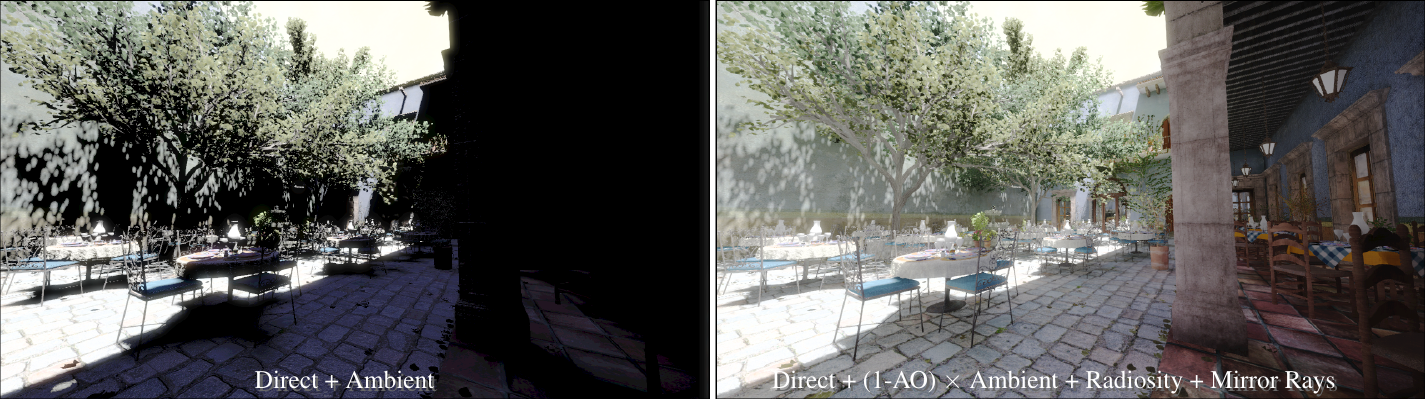
\includegraphics[width=\textwidth]{img/deep_g_buffer_render.png}
		\begin{itemize}
			\item 1920x1080 resolution
			\item rendered using NVIDIA GeForce 980
			\item in 10.8ms (92 FPS)
			\item looks good
		\end{itemize}
	\end{frame}

\end{document}